\index{general}{Mixed Formulation}
\begin{flushright} {\tiny {\color{gray} mixed.tex}} \end{flushright}

\subsection{In three dimensions}

The FEM formulation of the Stokes equation is quite complex so 
we simplify things as much as possible for now by 
assuming the flow to be \underline{incompressible}, 
\underline{isoviscous} and \underline{isothermal}. 

The methodology to derive the discretised equations of the mixed system is 
quite similar to the one we have used in the case of the penalty formulation.
The big difference comes from the fact that we are now solving for both 
velocity and pressure at the same time, and that we therefore must solve 
the mass and momentum conservation equations together.
As before, velocity inside an element is given by 
\begin{equation}
{\vec \upnu}^h({\vec r})=\sum_{i=1}^{m_v} \bN_i^\upnu({\vec r})\;  {\vec \upnu}_i
\label{mixed01}
\end{equation}
where $N_i^{\upnu}$ are the polynomial basis functions for the velocity,
and the summation runs over the $m_v$ velocity nodes composing the element.
A similar expression is used for pressure:
\begin{equation}
p^h({\vec r})=\sum_{i=1}^{m_p} \bN_i^p({\vec r}) \; p_i
\label{mixed02}
\end{equation}
Note that the velocity is a vector while pressure (and temperature)
is a scalar. There are then $ndof_v=ndim$ velocity degrees of freedom per node
and $ndof_p=1$ pressure degrees of freedom.
It is also very important to remember that the numbers of 
velocity nodes and pressure nodes for a given element 
are more often than not different and that velocity and pressure
nodes need not be colocated. Indeed, unless 
so-called 'stabilised elements' are used, we have $m_v>m_p$, which 
means that the polynomial order of the velocity field is higher than 
the polynomial order of the pressure field (usually by value 1).

Other notations will be sometimes used for Eqs.~\eqref{mixed01} and \eqref{mixed02}:
\begin{equation}
u^h({\vec r}) = \vec{\bN}^\upnu \cdot \vec{u}
\quad\quad\quad\quad
v^h({\vec r}) = \vec{\bN}^\upnu \cdot \vec{v}
\quad\quad\quad\quad
w^h({\vec r}) = \vec{\bN}^\upnu \cdot \vec{w}
\quad\quad\quad\quad
p^h({\vec r}) = \vec{\bN}^p \cdot \vec{p}
\end{equation} 
where ${\vec \upnu}=(u,v,w)$ and $\vec{\bN}^\upnu$ is the vector containing 
all basis functions evaluated at location ${\vec r}$:
\begin{eqnarray}
\vec{\bN}^v &=& \left( \bN_1^\upnu({\vec r}),  \bN_2^\upnu({\vec r}),  
\bN_3^\upnu({\vec r}), \dots  \bN_{m_v}^\upnu({\vec r}) \right) \\
\vec{\bN}^p &=& \left( \bN_1^p({\vec r}),  \bN_2^p({\vec r}),  
\bN_3^p({\vec r}), \dots  \bN_{m_p}^p({\vec r}) \right)
\end{eqnarray}
and with 
\begin{eqnarray}
\vec{u} &=& \left( u_1,  u_2,  u_3, \dots  u_{m_v} \right) \\
\vec{v} &=& \left( v_1,  v_2,  v_3, \dots  v_{m_v} \right) \\
\vec{w} &=& \left( w_1,  w_2,  w_3, \dots  w_{m_v} \right) \\
\vec{p} &=& \left( p_1,  p_2,  p_3, \dots  p_{m_p} \right) 
\end{eqnarray}
We will now establish the weak form of the momentum conservation equation. 
We start again from 
\begin{eqnarray}
{\vec \nabla}\cdot {\bm \sigma} + {\vec b} &=& {\vec 0} \\
{\vec \nabla}\cdot {\vec \upnu} &=& 0
\end{eqnarray}
For the $\bN_i^\upnu$'s and $\bN_i^p$ 'regular enough', we can write:
\begin{eqnarray}
\int_{\Omega_e} \bN_i^\upnu {\vec \nabla}\cdot {\bm \sigma}\;  dV
+ \int_{\Omega_e} \bN_i^\upnu  {\vec b} \; dV
&=& \vec 0 \\
\int_{\Omega_e} \bN_i^p {\vec \nabla}\cdot {\vec v} \; dV &=& 0
\end{eqnarray}
We can integrate by parts and drop the surface term\footnote{We will come back to this at a later stage}:
\begin{eqnarray}
\int_{\Omega_e} {\vec \nabla } \bN_i^\upnu \cdot {\bm \sigma} dV
&=& \int_{\Omega_e} \bN_i^\upnu  {\vec b} \; dV \\
\int_{\Omega_e} \bN_i^p {\vec \nabla}\cdot {\vec v} \; dV &=& 0
\end{eqnarray}
or, 
\begin{equation}
\int_{\Omega_e} 
\left(
\begin{array}{cccccc}
\frac{\partial \bN_i^\upnu}{\partial x} & 0 & 0& 
\frac{\partial \bN_i^\upnu}{\partial y} & 
\frac{\partial \bN_i^\upnu}{\partial z} & 0\\  \\
0 & \frac{\partial \bN_i^\upnu}{\partial y} & 0  & 
\frac{\partial \bN_i^\upnu}{\partial x}  & 0 &
\frac{\partial \bN_i^\upnu}{\partial z}  \\ \\
0 & 0 & \frac{\partial \bN_i^\upnu}{\partial z} &  0 & 
\frac{\partial \bN_i^\upnu}{\partial x} &  
\frac{\partial \bN_i^\upnu}{\partial y} 
\end{array}
\right)
\cdot
\left(
\begin{array}{c}
\sigma_{xx}\\
\sigma_{yy}\\
\sigma_{zz}\\
\sigma_{xy}\\
\sigma_{xz}\\
\sigma_{yz}\\
\end{array}
\right)
d\Omega = \int_{\Omega_e} \bN_i^\upnu {\vec b} \; dV
\end{equation}
The above equation can ultimately be written:
\begin{equation}
\int_{\Omega_e} {\bm B}^T \cdot 
\left(
\begin{array}{c}
\sigma_{xx}\\
\sigma_{yy}\\
\sigma_{zz}\\
\sigma_{xy}\\
\sigma_{xz}\\
\sigma_{yz}
\end{array}
\right)
dV
=
\int_{\Omega_e} {\vec \bN}_b\; dV
\end{equation}
We have previously established that the strain rate 
vector $\vec{\dot \varepsilon}$ is:
\begin{equation}
\vec{\dot\varepsilon}=
\left(
\begin{array}{c}
\frac{\partial u}{\partial x} \\ \\
\frac{\partial v}{\partial y} \\ \\
\frac{\partial w}{\partial z} \\ \\
\frac{\partial u}{\partial y}\! +\! \frac{\partial v}{\partial x} \\ \\
\frac{\partial u}{\partial z}\! +\! \frac{\partial w}{\partial x} \\ \\
\frac{\partial v}{\partial z}\! +\! \frac{\partial w}{\partial y} 
\end{array}
\right)
=
\left(
\begin{array}{c}
\sum\limits_i \frac{\partial \bN_i^\upnu}{\partial x} u_i \\ \\
\sum\limits_i \frac{\partial \bN_i^\upnu}{\partial y} v_i \\ \\
\sum\limits_i \frac{\partial \bN_i^\upnu}{\partial z} w_i \\ \\
\sum\limits_i (\frac{\partial \bN_i^\upnu}{\partial y} u_i\! +\! 
\frac{\partial \bN_i^\upnu}{\partial x} v_i) \\ \\
\sum\limits_i (\frac{\partial \bN_i^\upnu}{\partial z} u_i\! +\! 
\frac{\partial \bN_i^\upnu}{\partial x} w_i) \\ \\
\sum\limits_i (\frac{\partial \bN_i^\upnu}{\partial z} v_i\! +\! 
\frac{\partial \bN_i^\upnu}{\partial y} w_i) 
\end{array}
\right)
=
\underbrace{
\left(
\begin{array}{ccccccccccc}
\frac{\partial \bN_1^\upnu}{\partial x} & 0 & 0 &  \cdots  & 
\frac{\partial \bN_{m_v}^\upnu}{\partial x} & 0 & 0 \\ \\
0 & \frac{\partial \bN_1^\upnu}{\partial y} & 0 & \cdots & 0 & 
\frac{\partial \bN_{m_v}^\upnu}{\partial y} & 0 \\ \\
0 & 0 & \frac{\partial \bN_1^\upnu}{\partial z} & \cdots & 0 & 0 & 
\frac{\partial \bN_{m_v}^\upnu}{\partial z} 
\\ \\
\frac{\partial \bN_1^\upnu}{\partial y} &  \frac{\partial \bN_1^\upnu}{\partial x} &  
0 & \cdots  &\frac{\partial N_{m_v}^\upnu}{\partial x} 
& \frac{\partial \bN_{m_v}^\upnu}{\partial x} & 0 \\ \\
\frac{\partial \bN_1^\upnu}{\partial z} & 0 & \frac{\partial \bN_1^\upnu}{\partial x} & \cdots &
\frac{\partial \bN_{m_v}^\upnu}{\partial z} & 0 & \frac{\partial \bN_{m_v}^\upnu}{\partial x} \\  \\
0 &  \frac{\partial \bN_1^\upnu}{\partial z}  & \frac{\partial \bN_1^\upnu}{\partial y} & \cdots &
0 &  \frac{\partial \bN_{m_v}^\upnu}{\partial z}  & \frac{\partial \bN_{m_v}^\upnu}{\partial y} 
\end{array}
\right) 
}_{\bm B}
\!
\cdot
\!
\underbrace{
\left(
\begin{array}{c}
u_1 \\ v_1 \\ w_1 \\ u_2 \\ v_2 \\ w_2 \\ u_3 \\ v_3 \\ \dots \\ u_{m_v} \\ v_{m_v} \\ w_{m_v}
\end{array}
\right)
}_{\vec{\cal V}}
\end{equation}
or, $\vec{\dot \varepsilon}={\bm B}\cdot \vec{\cal V}$ where ${\bm B}$ is the gradient 
matrix and $\vec{\cal V}$ is the vector of all velocity degrees of freedom for the 
element. The matrix ${\bm B}$ is then of size $6 \times (m_v\cdot ndof_v) $ and the vector
$\vec{\cal V}$ is $m_v \cdot ndof_v$ long.
we have 
\begin{eqnarray}
\sigma_{xx}&=&-p + 2\eta \dot\varepsilon_{xx}^d \\
\sigma_{yy}&=&-p + 2\eta \dot\varepsilon_{yy}^d \\
\sigma_{zz}&=&-p + 2\eta \dot\varepsilon_{zz}^d \\
\sigma_{xy}&=& \hspace{8.5mm}  2\eta \dot\varepsilon_{xy}^d \\
\sigma_{xz}&=& \hspace{8.5mm}  2\eta \dot\varepsilon_{xz}^d \\
\sigma_{yz}&=& \hspace{8.5mm}  2\eta \dot\varepsilon_{yz}^d 
\end{eqnarray}
Since we here only consider incompressible flow, we have $\dot{\bm \varepsilon}^d=\dot{\bm \varepsilon}$
so
\begin{equation}
\vec{\sigma} 
=-\left( 
\begin{array}{c}
1 \\ 1 \\ 1 \\ 0 \\ 0 \\ 0
\end{array}
\right) p+ {\bm C} \cdot \vec{\dot\varepsilon}
=
- \left(
\begin{array}{c}
1 \\ 1 \\ 1 \\ 0 \\ 0 \\ 0
\end{array}
\right)
\vec{N^p} \cdot {\vec P}  + 
{\bm C} \cdot  {\bm B}\cdot {\vec V}
\end{equation}
with
\begin{equation}
{\bm C}=
\eta
\left(
\begin{array}{cccccc}
2 & 0 & 0 & 0 & 0 & 0\\
0 & 2 & 0 & 0 & 0 & 0\\
0 & 0 & 2 & 0 & 0 & 0\\ 
0 & 0 & 0 & 1 & 0 & 0\\ 
0 & 0 & 0 & 0 & 1 & 0\\ 
0 & 0 & 0 & 0 & 0 & 1
\end{array}
\right)
\quad\quad\quad
\vec{\dot \varepsilon} = 
\left(
\begin{array}{c}
\dot \varepsilon_{xx} \\
\dot \varepsilon_{yy} \\
\dot \varepsilon_{zz} \\
2\dot \varepsilon_{xy}\\ 
2\dot \varepsilon_{xz} \\
2\dot \varepsilon_{yz} 
\end{array}
\right)  \label{eq:mixedC}
\end{equation}
Let us define matrix ${\bm \bN}^p$ of size $6\times m_p$:
\begin{equation}
{\bm \bN}^p=
\left(
\begin{array}{c}
1 \\ 1 \\ 1 \\ 0 \\ 0 \\ 0
\end{array}
\right)
\vec{\bN^p} 
=
\left(
\begin{array}{c}
\vec{\bN^p} \\
\vec{\bN^p} \\
\vec{\bN^p} \\
0 \\
0 \\
0
\end{array}
\right)
\end{equation}
so that
\begin{equation}
\vec{\sigma} 
= - {\bm \bN}^p
 \cdot {\vec P}  + 
{\bm C} \cdot  {\bm B}\cdot {\vec V}
\end{equation}
finally
\begin{equation}
\int_{\Omega_e} {\bm B}^T \cdot 
[
- {\bm \bN}^p  \cdot {\vec P}  + {\bm C} \cdot  {\bm B}\cdot {\vec V}
]
\; d\Omega
=
\int_{\Omega_e} {\bm \bN}_b \; d\Omega 
\end{equation}
or,
\begin{equation}
\underbrace{\left(-\int_{\Omega_e} {\bm B}^T \cdot 
{\bm \bN}^p  
\; d\Omega \right)}_{\G} \cdot {\vec P} 
+
\underbrace{
\left(
\int_{\Omega_e} {\bm B}^T \cdot 
{\bm C} \cdot  {\bm B}
\; d\Omega
\right)}_{\K}
\cdot {\vec V}
=
\underbrace{\int_{\Omega_e} {\vec \bN}_b \; d\Omega }_{\vec f}
\end{equation}
where the matrix $\K$ is of size $(m_v \cdot ndof_v \times m_v \cdot ndof_v)$, 
and matrix ${\G}$ is of size $(m_v \cdot ndof_v \times m_p \cdot ndof_p)$.
Turning now to the mass conservation equation:
\begin{eqnarray}
\vec 0&=&\int_{\Omega_e} \vec{\bN}^p {\vec \nabla}\cdot {\vec v} \; d\Omega \nonumber\\
&=& \int_{\Omega_e} \vec{\bN}^p \sum_{i=1}^{m_v} 
\left( \frac{\partial \bN_i^\upnu}{\partial x} u_i + \frac{\partial \bN_i^\upnu}{\partial y} v_i 
+ \frac{\partial \bN_i^\upnu}{\partial z} w_i 
\right)  
d\Omega \nonumber\\
&=& 
\int_{\Omega_e} 
\left(
\begin{array}{c}
\bN_1^p \left(
\sum\limits_{i=1}^{m_v} \frac{\partial \bN_i^\upnu}{\partial x} u_i +
\sum\limits_{i=1}^{m_v} \frac{\partial \bN_i^\upnu}{\partial y} v_i +
\sum\limits_{i=1}^{m_v} \frac{\partial \bN_i^\upnu}{\partial z} w_i  \right) \\
\bN_2^p \left(
\sum\limits_{i=1}^{m_v} \frac{\partial \bN_i^\upnu}{\partial x} u_i +
\sum\limits_{i=1}^{m_v} \frac{\partial \bN_i^\upnu}{\partial y} v_i +
\sum\limits_{i=1}^{m_v} \frac{\partial \bN_i^\upnu}{\partial z} w_i  \right) \\
\bN_3^p \left(
\sum\limits_{i=1}^{m_v} \frac{\partial \bN_i^\upnu}{\partial x} u_i +
\sum\limits_{i=1}^{m_v} \frac{\partial \bN_i^\upnu}{\partial y} v_i +
\sum\limits_{i=1}^{m_v} \frac{\partial \bN_i^\upnu}{\partial z} w_i  \right) \\
\dots \\
\bN_{m_p}^p \left(
\sum\limits_{i=1}^{m_v} \frac{\partial \bN_i^\upnu}{\partial x} u_i +
\sum\limits_{i=1}^{m_v} \frac{\partial \bN_i^\upnu}{\partial y} v_i +
\sum\limits_{i=1}^{m_v} \frac{\partial \bN_i^\upnu}{\partial z} w_i  \right) 
\end{array}
\right) dV \nonumber \\  %%%%%%%%%%%%%%%%%%%%%%%%%%
&=& 
\int_{\Omega_e} 
\left(
\begin{array}{cccccc}
{\bN}_1^p & {\bN}_1^p & {\bN}_1^p & 0 & 0 & 0 \\\\
{\bN}_2^p & {\bN}_2^p & {\bN}_2^p & 0 & 0 & 0 \\\\
{\bN}_3^p & {\bN}_3^p & {\bN}_3^p & 0 & 0 & 0 \\\\
\vdots & \vdots & \vdots & \vdots & \vdots & \vdots \\\\
{\bN}_{m_p}^p & {\bN}_{m_p}^p & {\bN}_{m_p}^p & 0 &0 & 0 
\end{array}
\right)
\cdot
\left(
\begin{array}{c}
\sum\limits_i \frac{\partial \bN_i^\upnu}{\partial x} u_i \\ \\
\sum\limits_i \frac{\partial \bN_i^\upnu}{\partial y} v_i \\ \\
\sum\limits_i \frac{\partial \bN_i^\upnu}{\partial z} w_i \\ \\
\sum\limits_i (\frac{\partial \bN_i^\upnu}{\partial y} u_i\! +\! 
\frac{\partial \bN_i^\upnu}{\partial x} v_i) \\ \\
\sum\limits_i (\frac{\partial \bN_i^\upnu}{\partial z} u_i\! +\! 
\frac{\partial \bN_i^\upnu}{\partial x} w_i) \\ \\
\sum\limits_i (\frac{\partial \bN_i^\upnu}{\partial z} v_i\! +\! 
\frac{\partial \bN_i^\upnu}{\partial y} w_i) 
\end{array}
\right)
\; dV \nonumber\\ %%%%%%%%%%%%%%%%%%%%%%%%%%
&=& 
\int_{\Omega_e} 
\underbrace{
\left(
\begin{array}{cccccc}
{\bN}_1^p & {\bN}_1^p & {\bN}_1^p & 0 & 0 & 0 \\
{\bN}_2^p & {\bN}_2^p & {\bN}_2^p & 0 & 0 & 0 \\
{\bN}_3^p & {\bN}_3^p & {\bN}_3^p & 0 & 0 & 0 \\
\vdots & \vdots & \vdots & \vdots & \vdots & \vdots \\
{\bN}_{m_p}^p & {\bN}_{m_p}^p & {\bN}_{m_p}^p & 0 &0 & 0 
\end{array}
\right)
}_{({\bm \bN}^p)^T}
\cdot
\vec{\dot \varepsilon} \; dV  \nonumber \\
&=& 
\left(\int ({\bm \bN}^p)^T \cdot {\bm B} \; dV \right) \cdot \vec{V} \nonumber\\
&=& -\G_e^T \cdot {\vec V}
\end{eqnarray}

Note that it is common to actually start from $- \vec\nabla\cdot\vec v=0$ (see Eq.(3) in \cite{mabl14})
so as to arrive at $\G_e^T \cdot {\vec V}=\vec 0$


Ultimately we obtain the following system for each element:
\[
\left(
\begin{array}{cc}
\K_e & \G_e \\
-\G_e^T & 0
\end{array}
\right)
\cdot
\left(
\begin{array}{c}
\vec{V} \\ \vec{P} 
\end{array}
\right)
=
\left(
\begin{array}{c}
\vec{f}_e \\ 0 
\end{array}
\right)
\]
Such a matrix is then generated for each element and then must me assembled into the 
global F.E. matrix. 
Note that in this case the elemental Stokes matrix is antisymmetric. 
One can also define the following symmetric modified Stokes matrix:
\begin{equation}
\left(
\begin{array}{cc}
\K_e & \G_e \\
\G_e^T & 0
\end{array}
\right)
\cdot
\left(
\begin{array}{c}
\vec{V} \\ \vec{P} 
\end{array}
\right)
=
\left(
\begin{array}{c}
\vec{f}_e \\ 0 
\end{array}
\right)
\label{eq:KGGT}
\end{equation}
This matrix is symmetric, but indefinite. It is non-singular 
if $ker(\mathbb{G}^T)={ 0}$, which is the case if 
the compatibility condition holds.





{\color{red} CHECK:}
Matrix $\mathbb{K}$ is the viscosity matrix. Its size is $(ndof_v * N_v)\times (ndof_v * N_v)$ where $ndof_v$ is the number of velocity degrees of freedom per node (typically 1,2 or 3) and $N_v$ is the number of velocity nodes.
The size of matrix $\mathbb{G}$ is $(ndof_v * N_v)\times (ndof_p * N_p)$ where $ndof_p(=1)$  is the number of velocity degrees of freedom per node and $N_p$ is the number of pressure nodes. Conversely, the size of matrix $\mathbb{G}^T$ is $(ndof_p * N_p)\times (ndof_v * N_v)$.
The size of the global FE matrix is $N = ndof_v * N_v + ndof_p * N_p$
Note that matrix $\mathbb{K}$ is analogous to a discrete Laplacian operator, matrix $\mathbb{G}$ to a discrete gradient operator, and matrix $\mathbb{G}^T$ to a discrete divergence operator.





%--------------------------------------------------------------------------------
\subsubsection{On the physical dimensions of the Stokes matrix blocks}
We start from the Stokes equations:

\begin{eqnarray}
- {\vec \nabla p} + {\vec \nabla} \cdot (2 \eta \dot{\bm \varepsilon} ) + \rho \vec{g} &=& \vec{0}  \\
\vec \nabla \cdot \vec \upnu &=& 0 
\end{eqnarray}
We have
$[p]=ML^{-1}T^{-2}$, $[\vec\nabla]=L^{-1}$, so the dimensions of the terms in the first equation 
are: $ML^{-2}T^{-2}$. The blocks $\K$ and $\G$
stem from the weak form which is obtained by multiplying the strong form equations by the (dimensionless)
basis functions and integrating over the 3D domain, so that it follows that 
\[
[ \K \cdot \vec {\cal V}] = [\G \cdot \vec {\cal P}] = [\vec f] = (ML^{-2}T^{-2}) \cdot  L^3 = MLT^{-2} 
\]
We can then easily deduce:
\[
[\K]=MT^{-1}
\quad
\quad
[\G]=L^2
\]
%and finally this also imposes that $[\G^T V]= L^3T^{-1} $, and also that $[\C P]=L^3T^{-1} $,
%i.e. $[\C]=M^{-1}L^4T$ (analogous to $h^3/\mu$, which is also the dimension of the Schur
%complement $\SSS$). One can easily verify that $[\G^T \K \G]=[\C]$.

Turning to the mass conservation equation, we have $[\vec \nabla \cdot \vec \upnu]=L^{-1}LT^{-1}=T^{-1}$, 
which yields the discretised weak form $\G \cdot \vec{\cal V}=0$ so that $[\G \cdot \vec{\cal V}]=L^3 T^{-1}$ and
we of course recover $[\G]=L^2$.

If we wanted both equations to have the same dimensions, we would need to multiply the second one by a 
characteristic quantity which dimension is $M L^{-2} T^{-1}$, i.e. for example $\eta/L$ (since $[\eta]=ML^{-1}T^{-1}$).
This is indeed what we end up doing in practice, see Section~\ref{pscaling}.
   

%--------------------------------------------------------------------------------
\subsubsection{On elemental level mass balance}
Note that in what is above no assumption has been made about whether 
the pressure basis functions are continuous or discontinuous from one 
element to another. 

Indeed, as mentioned in Gresho \& Sani \cite{grsa}, since the 
weak formulation of the momentum equation involves
integration by parts of ${\vec \nabla }p$, the resulting weak form contains 
no derivatives of pressure. This introduces the possibility of approximating it
by functions (piecewise polynomials, of course) that are not $C^0$-continuous, 
and indeed this has been done and is quite popular/useful (e.g. $P_0$ or $P_{-1}$). 

It is then worth noting that {\sl only} discontinuous pressure 
elements assure an element-level mass balance \cite{grsa}:
if for instance $\bN_i^p$ is piecewise-constant on element $e$ (of value 1), the 
elemental weak form of the mass conservation equation is 
\[
\int_{\Omega_e} N_i^p {\vec \nabla} \cdot {\vec \upnu} = 
\int_{\Omega_e} {\vec \nabla} \cdot {\vec \upnu} = 
\int_{\Gamma_e} {\vec n} \cdot {\vec \upnu} = 0
\]
One potentially unwelcome consequence of using 
discontinuous pressure elements is that they 
do not possess uniquely defined pressure 
on the element boundaries; they are dual valued there, 
and often multi-valued at certain velocity nodes. 

%--------------------------------------------------------------------------------
\subsubsection{On the ${\bm C}$ matrix}

The relationship between deviatoric stress and deviatoric strain rate tensor is 
\begin{eqnarray}
\bm \tau 
&=& 2 \eta \dot{\bm \varepsilon}^d \\
&=& 2 \eta \left( \dot{\bm \varepsilon} -\frac{1}{3}(\vec\nabla\cdot\vec \upnu) {\bm 1} \right) \\
&=& 2 \eta
\left[ 
\left(
\begin{array}{ccc}
\dot\varepsilon_{xx} & \dot\varepsilon_{xy} & \dot\varepsilon_{xz} \\ 
\dot\varepsilon_{yx} & \dot\varepsilon_{yy} & \dot\varepsilon_{yz} \\ 
\dot\varepsilon_{zx} & \dot\varepsilon_{zy} & \dot\varepsilon_{zz} 
\end{array}
\right)
-
\frac{1}{3}
(\dot\varepsilon_{xx} + \dot\varepsilon_{yy} +  \dot\varepsilon_{zz})
\left(
\begin{array}{ccc}
1 &0 &0 \\
0 &1 &0\\ 
0 &0 &1 
\end{array}
\right)
\right] \\
&=& \frac{2}{3} \eta
\left(
\begin{array}{ccc}
2\dot\varepsilon_{xx} -\dot\varepsilon_{yy} -\dot\varepsilon_{zz} & 
3\dot\varepsilon_{xy} &
3\dot\varepsilon_{xz} \\ 
3\dot\varepsilon_{yx} & 
-\dot\varepsilon_{yy} +2\dot\varepsilon_{yy} -\dot\varepsilon_{yy} & 
3\dot\varepsilon_{yz} \\ 
3\dot\varepsilon_{zx} & 
3\dot\varepsilon_{zy} & 
-\dot\varepsilon_{xx} -\dot\varepsilon_{yy} + 2\dot\varepsilon_{zz}  
\end{array}
\right)
\end{eqnarray}
so that 
\begin{equation}
\vec \tau  
= \frac{2}{3} \eta
\left(
\begin{array}{c}
2\dot\varepsilon_{xx} -\dot\varepsilon_{yy} -\dot\varepsilon_{zz} \\ 
-\dot\varepsilon_{yy} +2\dot\varepsilon_{yy} -\dot\varepsilon_{yy} \\ 
-\dot\varepsilon_{xx} -\dot\varepsilon_{yy} +2\dot\varepsilon_{zz} \\
3\dot\varepsilon_{xy} \\
3\dot\varepsilon_{xz} \\
3\dot\varepsilon_{yz} 
\end{array}
\right)
=
\underbrace{
\frac{\eta}{3}
\left(
\begin{array}{cccccc}
4 & -2& -2& 0& 0& 0\\
-2 & 4& -2& 0& 0& 0\\
-2 & -2& 4& 0& 0& 0\\
0 &0 &0 & 3& 0& 0\\
0 &0 &0 & 0& 3& 0\\
0 &0 &0 & 0& 0& 3 
\end{array}
\right)
}_{{\bm C}^d}
\cdot
\left(
\begin{array}{c}
\dot\varepsilon_{xx} \\
\dot\varepsilon_{yy} \\
\dot\varepsilon_{zz} \\
2\dot\varepsilon_{xy} \\
2\dot\varepsilon_{xz} \\
2\dot\varepsilon_{yz} 
\end{array}
\right)
=
{\bm C}^d \cdot \vec{\dot \varepsilon}
\label{eq:chap6:mixed:Cd}
\end{equation}
which is identical to the one in the Appendix A of Schmalholz (2008) \cite{schm08}.
In two dimensions, we have
\[
\vec\tau=\frac{1}{3}\eta 
\underbrace{
\left(
\begin{array}{ccc}
4 & -2 & 0 \\
-2 & 4 & 0 \\
0 &0 &  3 
\end{array}
\right)
}_{{\bm C}^d}
\cdot
\]
see for instance Andres-Martinez \etal (2015) \cite{anmp15}.

In the case where we assume incompressible flow from the beginning, 
i.e. $\dot{\bm \varepsilon}=\dot{\bm \varepsilon}^d$, 
then 
\begin{equation}
\vec \tau  
=
\underbrace{
\eta
\left(
\begin{array}{cccccc}
2 & 0& 0& 0& 0& 0\\
0 & 2& 0& 0& 0& 0\\
0 & 0& 2& 0& 0& 0\\
0 &0 &0 & 1& 0& 0\\
0 &0 &0 & 0& 1& 0\\
0 &0 &0 & 0& 0& 1 
\end{array}
\right)
}_{\bm C}
\cdot
\left(
\begin{array}{c}
\dot\varepsilon_{xx} \\
\dot\varepsilon_{yy} \\
\dot\varepsilon_{zz} \\
2\dot\varepsilon_{xy} \\
2\dot\varepsilon_{xz} \\
2\dot\varepsilon_{yz} 
\end{array}
\right)
=
{\bm C} \cdot \vec{\dot \varepsilon}
\end{equation}

%--------------------------------------------------------------------------------
\subsubsection{A slightly different formulation}

The momentum conservation equation can be written as follows:
\[
\vec\nabla\cdot( 2 \eta \dot{\bm \varepsilon}(\vec\upnu)) - \vec\nabla p + \vec b = \vec 0
\]
When the viscosity $\eta$ is constant and the flow is incompressible this equation becomes
\[
\eta \Delta \vec \upnu - \vec\nabla p + \vec b = \vec 0
\]
In this case the matrix ${\bm B}$ takes a different form (See Donea \& Huerta \cite[Eq. 6.24]{dohu03})
and one should be aware that this can have consequences for the Neumann boundary conditions. 

In Burstedde \etal (2009) \cite{bugs09} the authors state that when the Laplacian formulation is used 
it has the computational advantage that the velocity
components are coupled only through the incompressibility condition. 
While the two formulations are equivalent only for constant viscosity, they state 
that they employ the Laplacian approach formulation as a preconditioner for the viscous term. 

Concretely, we apply the same method as above, i.e. we reorganise the terms of the 
velocity gradient tensor in a vector:
\begin{eqnarray}
\vec\nabla \vec\upnu 
&\rightarrow &
\left(
\begin{array}{c}
\partial_x u \\
\partial_y u \\
\partial_z u \\
\partial_x v \\
\partial_y v \\
\partial_z v \\
\partial_x w \\
\partial_y w \\
\partial_z w 
\end{array}
\right)
=
\left(
\begin{array}{c}
\sum_i \partial_x \bN_i u_i \\
\sum_i \partial_y \bN_i u_i \\
\sum_i \partial_z \bN_i u_i \\
\sum_i \partial_x \bN_i v_i \\
\sum_i \partial_y \bN_i v_i \\
\sum_i \partial_z \bN_i v_i \\
\sum_i \partial_x \bN_i w_i \\
\sum_i \partial_y \bN_i w_i \\
\sum_i \partial_z \bN_i w_i 
\end{array}
\right) \nonumber\\
&=&
\underbrace{
\left(
\begin{array}{cccccccccc}
\partial_x \bN_1^\upnu & 0 & 0 & \partial_x \bN_2^\upnu & 0 & 0 & \cdots & \partial_x \bN^\upnu_{m_\upnu} & 0 & 0 \\
\partial_y \bN_1^\upnu & 0 & 0 & \partial_y \bN_2^\upnu & 0 & 0 & \cdots & \partial_y \bN^\upnu_{m_\upnu} & 0 & 0 \\
\partial_z \bN_1^\upnu & 0 & 0 & \partial_z \bN_2^\upnu & 0 & 0 & \cdots & \partial_z \bN^\upnu_{m_\upnu} & 0 & 0 \\
0 & \partial_x \bN_1^\upnu & 0 & 0& \partial_x \bN_2^\upnu & 0 & \cdots & 0 & \partial_x \bN^\upnu_{m_\upnu}  & 0 \\
0 & \partial_y \bN_1^\upnu & 0 & 0& \partial_y \bN_2^\upnu & 0 & \cdots & 0 & \partial_y \bN^\upnu_{m_\upnu}  & 0 \\
0 & \partial_z \bN_1^\upnu & 0 & 0& \partial_z \bN_2^\upnu & 0 & \cdots & 0 & \partial_z \bN^\upnu_{m_\upnu}  & 0 \\
0 & 0 & \partial_x \bN_1^\upnu  & 0& 0& \partial_x \bN_2^\upnu & \cdots & 0 & 0 & \partial_x \bN^\upnu_{m_\upnu}  \\
0 & 0 & \partial_y \bN_1^\upnu  & 0& 0& \partial_y \bN_2^\upnu & \cdots & 0 & 0 & \partial_y \bN^\upnu_{m_\upnu}  \\
0 & 0 & \partial_z \bN_1^\upnu  & 0& 0& \partial_z \bN_2^\upnu & \cdots & 0 & 0 & \partial_z \bN^\upnu_{m_\upnu}  \\
\end{array}
\right) 
}_{\bm B}
\!
\cdot
\!
\underbrace{
\left(
\begin{array}{c}
u_1 \\ v_1 \\ w_1 \\ u_2 \\ v_2 \\ w_2 \\ u_3 \\ v_3 \\ \dots \\ u_{m_v} \\ v_{m_v} \\ w_{m_v}
\end{array}
\right)
}_{\vec V} \nonumber
\end{eqnarray}
and in two dimensions:
\[
\vec\nabla \vec\upnu \rightarrow 
\left(
\begin{array}{c}
\partial_x u \\
\partial_y u \\
\partial_x v \\
\partial_y v 
\end{array}
\right)
=
\left(
\begin{array}{c}
\sum_i \partial_x \bN_i u_i \\
\sum_i \partial_y \bN_i u_i \\
\sum_i \partial_x \bN_i v_i \\
\sum_i \partial_y \bN_i v_i 
\end{array}
\right)
=
\underbrace{
\left(
\begin{array}{cccccccccc}
\partial_x \bN_1^\upnu & 0  & \partial_x \bN_2^\upnu & 0  & \cdots & \partial_x \bN_i^\upnu{m_\upnu} & 0 \\
\partial_y \bN_1^\upnu & 0  & \partial_y \bN_2^\upnu & 0  & \cdots & \partial_y \bN_i^\upnu{m_\upnu} & 0 \\
0 & \partial_x \bN_1^\upnu  & 0& \partial_x \bN_2^\upnu  & \cdots & 0 & \partial_x \bN_i^\upnu{m_\upnu}  \\
0 & \partial_y \bN_1^\upnu  & 0& \partial_y \bN_2^\upnu  & \cdots & 0 & \partial_y \bN_i^\upnu{m_\upnu}  
\end{array}
\right) 
}_{\bm B}
\cdot
\underbrace{
\left(
\begin{array}{c}
u_1 \\ v_1 \\ u_2 \\ v_2 \\ u_3 \\ v_3 \\ \dots \\ u_{m_v} \\ v_{m_v} 
\end{array}
\right)
}_{\vec V}
\]

If such a formulation is used, it makes more sense to actually group the unknowns as follows:
\[
\vec{\cal V}=(u_1, \dots, u_{m_\upnu},v_1,\dots,v_{m_\upnu}, w_1, \dots, w_{m_\upnu})
\]

We start from 
\[
\eta \Delta \vec\upnu -\vec\nabla p + \rho \vec{g} = \vec{0}
\]
In 2D Cartesian coordinates this becomes:
\begin{eqnarray}
\eta \Delta u - \partial_x p + \rho g_x &=& 0\\
\eta \Delta v - \partial_y p + \rho g_y &=& 0
\end{eqnarray}
or, 
\begin{eqnarray}
\eta \left(\frac{\partial^2 u}{\partial x^2} + \frac{\partial^2 u}{\partial y^2} \right) - \partial_x p + \rho g_x &=& 0\\
\eta \left(\frac{\partial^2 v}{\partial x^2} + \frac{\partial^2 v}{\partial y^2} \right) - \partial_y p + \rho g_y &=& 0
\end{eqnarray}
Assuming that we prescribe the normal velocity on all sides (i.e. no Neumann boundary conditions), we can establish the weak form of these equations:
\begin{eqnarray}
\underbrace{
\left(
\int_\Omega \eta (
\frac{\partial \vec{\bN}^\upnu}{\partial x}
\frac{\partial \vec{\bN}^\upnu}{\partial x} 
+
\frac{\partial \vec{\bN}^\upnu}{\partial y}
\frac{\partial \vec{\bN}^\upnu}{\partial y}) \;
dV \right) }_{\N}
\cdot \vec{\cal V}_x
+
\underbrace{
\left(
-\int_\Omega \frac{\partial \vec{\bN}^\upnu}{\partial x} \vec{\bN}^p \; dV
\right)}_{G_{x}}
\cdot \vec{\cal P} 
&=& \underbrace{ \int_\Omega \vec{\bN}^\upnu \rho g_x \; dV }_{\vec{f}_x}\\
\underbrace{
\left(
\int_\Omega \eta (
\frac{\partial \vec{\bN}^\upnu}{\partial x}
\frac{\partial \vec{\bN}^\upnu}{\partial x} 
+
\frac{\partial \vec{\bN}^\upnu}{\partial y}
\frac{\partial \vec{\bN}^\upnu}{\partial y}) \;
dV \right) }_{\N}
\cdot \vec{\cal V}_y
+
\underbrace{
\left(
-\int_\Omega \frac{\partial \vec{\bN}^\upnu}{\partial y} \vec{\bN}^p \; dV
\right)}_{G_{y}}
\cdot \vec{\cal P} 
&=& \underbrace{ \int_\Omega \vec{\bN}^\upnu \rho g_y \; dV }_{\vec{f}_y}
\end{eqnarray}
Turning now to the continuity equation
\[
-\vec\nabla\cdot\vec\upnu = 0
\]
or,
\[
-\frac{\partial u}{\partial x} 
-\frac{\partial v}{\partial y} =0
\]
Its weak form then is
\[
\underbrace{
\left(-\int_\Omega \vec{\bN}^p \frac{\partial \vec{\bN}^\upnu}{\partial x} dV
\right) \cdot \vec{\cal V}_x }_{G_x^T}
+
\underbrace{\left(- \int_\Omega \vec{\bN}^p \frac{\partial \vec{\bN}^\upnu}{\partial y}   dV \right)}_{G_y^T} \cdot \vec{\cal V}_y 
=0
\]
In the end:
\[
\left(
\begin{array}{ccc}
{\N} & 0 & {\G}_x  \\
0 & {\N} & {\G}_y  \\
\G_x & \G_y & 0 
\end{array}
\right)
\cdot
\left(
\begin{array}{c}
\vec{\cal V}_x \\
\vec{\cal V}_y \\
\vec{\cal P} 
\end{array}
\right)
=
\left(
\begin{array}{c}
\vec{f}_x \\
\vec{f}_y \\
0
\end{array}
\right)
\]

This approach is implemented in \stone~48. 






%-----------------------------------------------------------------------------------
\subsubsection{On the 'forgotten' surface terms}

FINISH write

%-----------------------------------------------------------------------------------
\subsection{Revisiting the penalty method}
\index{general}{Penalty Formulation}
\index{general}{Pressure Mass Matrix}

We have just seen that the discretised Stokes equation yield the 
following saddle point system:

%From \cite{segal}. In the discrete penalty function method,
%the (Navier-)stokes equations are discretized before applying
%the penalty function method. So we start with the formulation

\[
\left( \begin{array}{cc}
\K & \G  \\ 
\G^T & 0 
\end{array} \right) \cdot
\left( \begin{array}{c}  \vec{\cal V} \\ \vec{\cal P}  \end{array} \right) = 
\left( \begin{array}{c}  \vec{f} \\ \vec{0}  \end{array} \right) 
\]
One can perturb the continuity equation 
by a term $\C_\epsilon = \epsilon \mathbb{M}_p$
where $\mathbb{M}_p$ is the pressure mass matrix.
This yields
\[
\left( \begin{array}{cc}
\K & \G  \\ \G^T & -\mathbb{C}_\epsilon
\end{array} \right) \cdot
\left( \begin{array}{c}  \vec{\cal V} \\ \vec{\cal P}  \end{array} \right) = 
\left( \begin{array}{c}  \vec{f} \\ \vec{0}  \end{array} \right) 
\]
or,
\[
\vec{\cal P}= \frac{1}{\epsilon} \mathbb{M}_p^{-1} \cdot  \G^T \cdot \vec{\cal V}
\]
Substituting pressure in the first equation yields:
\begin{equation}
(\K + \frac{1}{\epsilon} \G \cdot \mathbb{M}_p^{-1} \cdot \G^T ) \cdot \vec{\cal V} = \vec{f} 
\label{eqdpf}
\end{equation}

If we want to solve these equations, it is necessary that the matrix $\mathbb{M}_p^{-1}$
can be computed easily.
This is for example the case if $\mathbb{M}_p$
is a lumped mass matrix (often done for Taylor-Hood elements). 
When discontinuous pressure elements are used,
$\mathbb{M}_p$ is in a block diagonal matrix, i.e. a diagonal matrix consisting of small matrices as diagonal elements. One can easily verify that these small matrices have the size of the number of pressure unknowns per element. Note that this is all carried out at the elemental level.

%Another practical aspect is that the building of the matrix $\mathbb{G} \mathbb{M}^{-1} \mathbb{G}^T$
%must be easy. Moreover, it would be very nice if this matrix could be built
%per element by element matrices. In that case the structures of ${\bm K}$
%and $\mathbb{G} \mathbb{M}^{-1} \mathbb{G}^T$ are identical and the solution of (\ref{eqdpf})
%is as simple as
%the solution of $\mathbb{K} {\bm u}={\bm f} $.




%--------------------------------------------------------------------------
\subsection{A much more compact derivation of the Stokes matrix blocks \label{sss:KGGT}}

What follows is inspired by chapter 6 of \textcite{dohu03}.
One can easily show that the weak form of the Stokes system can be written 
\begin{eqnarray}
\int_\Omega \vec\nabla \vec{\upomega} : {\bm \sigma} \; d\Omega
&=& \int_\Omega \vec\upomega \cdot \vec{b} \; d\Omega + \int_\Gamma \vec\upomega \cdot \vec{t} \; d\Gamma \\
\int_\Omega q \vec\nabla \cdot \vec{\upnu} \; d\Omega &=& 0
\end{eqnarray}
where $\vec\upomega$ and $q$ are the velocity and pressure test functions respectively, 
and with 
\[
\vec\nabla \vec{\upomega} :\ {\bm \sigma} 
= \sum_{i,j}^{ndim} \frac{\partial \upomega _i}{\partial x_j} \sigma_{ij}
\]
Assuming the Cauchy stress ${\bm \sigma}$ is given by the linear Stokes' law
${\bm \sigma} = -p {\bm 1} + {\bm \tau}$ with 
${\bm \tau} = 2\eta \dot{\bm \epsilon}(\vec\upnu) = {\cal C}: \vec\nabla\vec\upnu$
where ${\cal C}$ is a fourth-order tensor with 
${\cal C}_{ijkl} = \eta (\delta_{ik} \delta_{jl}+ \delta_{il}\delta_{jk})$. 
Then 
\begin{eqnarray}
\int_\Omega \vec\nabla \vec{\upomega} : {\bm \sigma} \; d\Omega
&=& \int_\Omega \vec\nabla \vec{\upomega} : ( -p {\bm 1} + {\bm \tau}) \; d\Omega \nonumber\\
&=& - \int_\Omega p \; \vec\nabla  \vec{\upomega} : {\bm 1}  \; d\Omega 
+ \int_\Omega \vec\nabla \vec{\upomega} : {\bm \tau} \; d\Omega \nonumber\\
&=& - \int_\Omega p \; \vec\nabla\cdot  \vec{\upomega}   \; d\Omega 
+ \int_\Omega \vec\nabla \vec{\upomega} : {\cal C} : \vec\nabla \vec\upnu\; d\Omega 
\end{eqnarray}
The weak form of the Stokes system now takes the form
\begin{eqnarray}
- \int_\Omega p \; \vec\nabla\cdot  \vec{\upomega}   \; d\Omega 
+ \int_\Omega \vec\nabla \vec{\upomega} : {\cal C} : \vec\nabla \vec\upnu\; d\Omega 
&=& \int_\Omega \vec\upomega \cdot \vec{b} \; d\Omega + \int_\Gamma \vec\upomega \cdot \vec{t} \; d\Gamma \\
\int_\Omega q \vec\nabla \cdot \vec{\upnu} \; d\Omega &=& 0
\end{eqnarray}
Actually, the bilinear form with the two double dot products is not particularly convenient so 
it is always rewritten in terms of the strain rate vector
\[
\vec{\dot \varepsilon}(\vec\upnu) = 
\left(
\begin{array}{c}
\dot \varepsilon_{xx}(\vec\upnu) \\
\dot \varepsilon_{yy}(\vec\upnu) \\
\dot \varepsilon_{zz}(\vec\upnu) \\
2\dot \varepsilon_{xy}(\vec\upnu)\\ 
2\dot \varepsilon_{xz}(\vec\upnu)\\
2\dot \varepsilon_{yz}(\vec\upnu) 
\end{array}
\right)
\]
as one can easily show that 
\[
\vec\nabla \vec{\upomega} : {\cal C} : \vec\nabla \vec\upnu = 
\vec{\dot \varepsilon}(\vec\upomega)^T \cdot {\bm C}_\eta \cdot \vec{\dot \varepsilon}(\vec\upnu)
\]
with 
\[
{\bm C}_\eta=
\eta
\left(
\begin{array}{cccccc}
2 & 0 & 0 & 0 & 0 & 0\\
0 & 2 & 0 & 0 & 0 & 0\\
0 & 0 & 2 & 0 & 0 & 0\\ 
0 & 0 & 0 & 1 & 0 & 0\\ 
0 & 0 & 0 & 0 & 1 & 0\\ 
0 & 0 & 0 & 0 & 0 & 1
\end{array}
\right)
\]
and since 
$\vec{\dot \varepsilon}(\vec\upnu) = {\bm B} \cdot \vec{\cal V}$
and
$\vec{\dot \varepsilon}(\vec\upomega) = {\bm B} \cdot \vec{\cal W}$
then
\begin{eqnarray}
\int_\Omega \vec\nabla\vec{\upomega} : {\cal C} : \vec\nabla \vec\upnu  \; d\Omega
&=& \int_\Omega
\vec{\dot \varepsilon}(\vec\upomega)^T \cdot {\bm C}_\eta \cdot \vec{\dot \varepsilon}(\vec\upnu) \; d\Omega \nonumber\\
&=& \int_\Omega
\vec{\cal W}^T \cdot {\bm B}^T \cdot {\bm C}_\eta \cdot {\bm B} \cdot \vec{\cal V} \; d\Omega \nonumber\\ 
&=& \vec{\cal W}^T \cdot \int_\Omega  {\bm B}^T \cdot {\bm C}_\eta \cdot {\bm B}  \; d\Omega \cdot \vec{\cal V} \nonumber\\
&=& \vec{\cal W}^T \cdot \mathbb{K} \cdot \vec{\cal V} 
\end{eqnarray}

Let us now turn to the mass conservation equation:
\[
\int_\Omega q \vec\nabla \cdot \vec{\upnu} \; d\Omega 
=\int_\Omega \vec{\cal Q}^T \vec{\cal N}^p \vec\nabla \cdot \vec{\upnu} \; d\Omega  
=\vec{\cal Q}^T \cdot \int_\Omega \vec{\cal N}^p \vec\nabla \cdot \vec{\upnu} \; d\Omega  
\]
We have $\vec\nabla \cdot \vec{\upnu} = Tr[\dot{\bm \varepsilon}(\vec\upnu)]$ but also 
\begin{eqnarray}
\vec\nabla \cdot \vec{\upnu} 
&=& 
\left(
\begin{array}{cccccc}
1 & 1 & 1 & 0 & 0 & 0
\end{array}
\right)
\cdot
\left(
\begin{array}{c}
\dot \varepsilon_{xx}(\vec\upnu) \\
\dot \varepsilon_{yy}(\vec\upnu) \\
\dot \varepsilon_{zz}(\vec\upnu) \\
2\dot \varepsilon_{xy}(\vec\upnu)\\ 
2\dot \varepsilon_{xz}(\vec\upnu)\\
2\dot \varepsilon_{yz}(\vec\upnu) 
\end{array}
\right) \nonumber\\
&=&
\left(
\begin{array}{cccccc}
1 & 1 & 1 & 0 & 0 & 0
\end{array}
\right)
\cdot
\vec{\dot \varepsilon}(\vec\upnu)  \nonumber\\
&=&
\left(
\begin{array}{cccccc}
1 & 1 & 1 & 0 & 0 & 0
\end{array}
\right)
\cdot
{\bm B} \cdot \vec{\cal V}
\end{eqnarray}
so that 
\begin{eqnarray}
\vec{\cal N}^p  \vec\nabla \cdot \vec{\upnu}
&=& \vec{\cal N}^p  
\left(
\begin{array}{cccccc}
1 & 1 & 1 & 0 & 0 & 0
\end{array}
\right)
\cdot
{\bm B} \cdot \vec{\cal V} \nonumber\\
&=&
\left(
\begin{array}{cccccc}
\vec{\cal N}^p & \vec{\cal N}^p & \vec{\cal N}^p & 0 & 0 & 0
\end{array}
\right)
\cdot
{\bm B} \cdot \vec{\cal V} \nonumber\\
&=&
{\bm \bN}^T \cdot {\bm B} \cdot \vec{\cal V}
\end{eqnarray}
Finally 
\begin{eqnarray}
\int_\Omega q \vec\nabla \cdot \vec{\upnu} \; d\Omega 
&=& \vec{\cal Q}^T \cdot \int_\Omega {\bm \bN}^T \cdot {\bm B} \; d\Omega \cdot \vec{\cal V} \nonumber\\
&=& - \vec{\cal Q}^T \cdot \mathbb{G}^T \cdot \vec{\cal V} 
\end{eqnarray}
where 
\[
\mathbb{G} = -\int_\Omega {\bm B}^T \cdot {\bm \bN}\; d\Omega 
\]

Obviously the term 
$- \int_\Omega p \; \vec\nabla  \vec{\upomega} : {\bm 1}  \; d\Omega 
=- \int_\Omega p \; \vec\nabla \cdot \vec{\upomega}   \; d\Omega $
will take the form
$\vec{\cal P}^T \cdot {\bm G}^T \cdot \vec{\cal W} = 
\vec{\cal W}^T \cdot {\bm G} \cdot \vec{\cal P} $
so that 

\[
- \int_\Omega p \; \vec\nabla\cdot  \vec{\upomega}   \; d\Omega 
+ \int_\Omega \vec\nabla \vec{\upomega} : {\cal C} : \vec\nabla \vec\upnu\; d\Omega 
=
\vec{\cal W}^T \cdot {\bm G} \cdot \vec{\cal P} 
+
\vec{\cal W}^T \cdot \mathbb{K} \cdot \vec{\cal V} 
=
\vec{\cal W}^T \cdot \left( {\bm G} \cdot \vec{\cal P} + \mathbb{K} \cdot \vec{\cal V} \right)
\]
The rhs are handled as shown previously. 
Since these relationships must work for any test function then
it means that what multiplies $\vec{\cal W}$ and $\vec{\cal Q}$ must be null
and we recover Eq.~\eqref{eq:KGGT}.

Note that this approach is quite versatile since it does not require to specify the 
coordinate system. The vector $\vec{\dot \varepsilon}$ will contain the components of the 
strain rate tensor and in the end the matrix ${\bm B}$ will reflect the exact 
form of the strain rate tensor terms (see axisymmetric formulation).


\subsection{Pressure scaling \label{pscaling}} 
\index{general}{pressure scaling}
\begin{flushright} {\tiny {\color{gray} pressure\_scaling.tex}} \end{flushright}
%~~~~~~~~~~~~~~~~~~~~~~~~~~~~~~~~~~~~~~~~~~~~~~~~~~~~~~~~~~~~~~~~~~~~~~~~~~~~~~~~~~~~~~~~~~~~~~~~~~

As nicely explained in the 
step 32 of deal.ii\footnote{\url{https://www.dealii.org/9.0.0/doxygen/deal.II/step\_32.html}},
we often need to scale the $\G$ block since it is many orders of magnitude smaller than $\K$ (especially in geodynamics where viscosities are $\sim 10^{22}$), 
which introduces large inaccuracies in the solving process to the point that the solution is nonsensical. 
This scaling coefficient is $\eta/L$ where $\eta$ and $L$ are representative viscosities and lengths. 
We start from 
\[
\left(
\begin{array}{cc}
\K & \G \\ \G^T & -\C 
\end{array}
\right)
\cdot
\left(
\begin{array}{c}
\vec{\cal V} \\ \vec{\cal P}
\end{array}
\right)
=
\left(
\begin{array}{c}
\vec{f} \\ \vec{h}
\end{array}
\right)
\]
and introduce the scaling coefficient as follows (which in fact does not alter the solution at all):
\[
\left(
\begin{array}{cc}
\K & \frac{\eta}{L}\G \\ \frac{\eta}{L}\G^T & - \frac{\eta^2}{L^2} \C 
\end{array}
\right)
\cdot
\left(
\begin{array}{c}
\vec{\cal V} \\\frac{L}{\eta} \vec{\cal P}
\end{array}
\right)
=
\left(
\begin{array}{c}
 \vec{f} \\ \frac{\eta}{L} \vec{h}
\end{array}
\right)
\]
We then end up with the modified Stokes system:
\[
\left(
\begin{array}{cc}
\K & \underline{\G} \\ \underline{\G}^T & \underline{\C} 
\end{array}
\right)
\cdot
\left(
\begin{array}{c}
\vec{\cal V} \\ \underline{\vec{\cal P}}
\end{array}
\right)
=
\left(
\begin{array}{c}
\vec{f} \\ \underline{\vec{h}}
\end{array}
\right)
\]
where 
\[
\underline{\G}=\frac{\eta}{L}\G
\quad\quad
\quad\quad
\underline{\vec{\cal P}}=\frac{L}{\eta} \vec{\cal P}
\quad\quad
\quad\quad
\underline{\C}=\frac{\eta^2}{L^2} \C
\quad\quad
\quad\quad
\underline{\vec{h}}=\frac{\eta}{L}\vec{h}
\]
After the solve phase, we recover the real pressure with $\vec{\cal P}=\frac{\eta}{L}\underline{\vec{\cal P}}$.





 %-----------------------------







%--------------------------------------------------------------------------------
\subsection{Going from 3D to 2D}

The world is three-dimensional. However, for many different reasons one may wish to solve problems
which are two-dimensional. 

Following ASPECT manual, we  will think of two-dimensional models in the following way: 
\begin{itemize}
\item We assume that the domain we want to solve on is a two-dimensional cross section (in the $x-y$ plane) 
that extends infinitely far in both negative and positive $z$ direction.  
\item We assume that the velocity is zero in the $z$ direction and that all variables 
have no variation in the $z$ direction. 
\end{itemize}

As a consequence, two-dimensional models are three-dimensional ones in which the $z$ 
component of the velocity is zero and so are all $z$ derivatives.
This allows to reduce the momentum conservation equations from 3 equations to 2 equations. 
However, contrarily to what is often seen, the 3D definition of the deviatoric strain rate 
remains, i.e. in other words:
\begin{equation}
\dot{\bm \varepsilon}^d = \dot{\bm \varepsilon} -\frac{1}{3}(\vec\nabla\cdot\vec v) {\bm 1} 
\end{equation}
and not $1/2$.
In light of all this, the full strain rate tensor and the 
deviatoric strain rate tensor in 2D are given by:

\begin{eqnarray}
{\bm \varepsilon}&=&
\left(
\begin{array}{ccc}
\dot\varepsilon_{xx} & \dot\varepsilon_{xy} & \dot\varepsilon_{xz} \\ 
\dot\varepsilon_{yx} & \dot\varepsilon_{yy} & \dot\varepsilon_{yz} \\ 
\dot\varepsilon_{zx} & \dot\varepsilon_{zy} & \dot\varepsilon_{zz} 
\end{array}
\right)
=
\left(
\begin{array}{ccc}
\frac{\partial u}{\partial x} & \frac{1}{2}\left(\frac{\partial u}{\partial y} + \frac{\partial v}{\partial x}\right)  & 0 \\
\frac{1}{2}\left(\frac{\partial u}{\partial y} + \frac{\partial v}{\partial x}\right)  &  \frac{\partial v}{\partial y} & 0 \\
0 & 0 & 0
\end{array}
\right) \\
\dot{\bm \varepsilon}^d &=&
\frac{1}{3}
\left(
\begin{array}{ccc}
2 \frac{\partial u}{\partial x} - \frac{\partial v}{\partial y} &  
 \frac{1}{2}\left(\frac{\partial u}{\partial y} + \frac{\partial v}{\partial x}\right) &
0 \\ 
 \frac{1}{2}\left(\frac{\partial u}{\partial y} + \frac{\partial v}{\partial x}\right) &
- \frac{\partial u}{\partial x} +2 \frac{\partial v}{\partial y} &  
0 \\ 
0 & 0 & -\frac{\partial u}{\partial x} - \frac{\partial v}{\partial y}
\end{array}
\right)
\end{eqnarray}
Although the bottom right term may be surprising, it is of no consequence when this expression of the deviatoric strain rate is used in the Stokes equation:
\[
{\vec \nabla} \cdot 2\eta \dot{\bm \varepsilon}^d
=
\]
{\color{red} FINISH!}

In two dimensions the velocity is then $\vec\upnu=(u,v)$ and the FEM building blocks and matrices are simply:
\begin{equation}
\vec{\dot\varepsilon}
=
\left(
\begin{array}{c}
\dot \varepsilon_{xx} \\\\
\dot \varepsilon_{yy} \\\\
2\dot \varepsilon_{xy} 
\end{array}
\right)
=
\left(
\begin{array}{c}
\frac{\partial u}{\partial x} \\ \\
\frac{\partial v}{\partial y} \\ \\
\frac{\partial u}{\partial y} + \frac{\partial v}{\partial x} \\
\end{array}
\right)
=
\underbrace{
\left(
\begin{array}{ccccccccccc}
\frac{\partial N_1^\upnu}{\partial x} & 0 & 
\frac{\partial N_2^\upnu}{\partial x} & 0 & 
\frac{\partial N_3^\upnu}{\partial x} & 0 & \dots & 
\frac{\partial N_{m_v}^\upnu}{\partial x} & 0
\\  \\
0 & \frac{\partial N_1^\upnu}{\partial y} & 
0 & \frac{\partial N_2^\upnu}{\partial y} &
0 & \frac{\partial N_3^\upnu}{\partial y} & \dots & 
0 & \frac{\partial N_{m_v}^\upnu}{\partial x} 
\\ \\
\frac{\partial N_1^\upnu}{\partial y} &  \frac{\partial N_1^\upnu}{\partial x} &  
\frac{\partial N_2^\upnu}{\partial y} &  \frac{\partial N_2^\upnu}{\partial x} & 
\frac{\partial N_3^\upnu}{\partial y} &  \frac{\partial N_3^\upnu}{\partial x} &   \dots &  
\frac{\partial N_{m_v}^\upnu}{\partial y} &  \frac{\partial N_{m_v}^\upnu}{\partial x}  
\end{array}
\right) 
}_{\bm B}
\cdot
\underbrace{
\left(
\begin{array}{c}
u_1 \\ v_1 \\ u_2 \\ v_2 \\ u_3 \\ v_3 \\ \dots \\ u_{m_v} \\ v_{m_v}
\end{array}
\right)
}_{\vec V}
\end{equation}

we have 
\begin{eqnarray}
\sigma_{xx}&=&-p + 2\eta \dot\varepsilon_{xx} \\
\sigma_{yy}&=&-p + 2\eta \dot\varepsilon_{yy} \\
\sigma_{xy}&=& \hspace{5.5mm} + 2\eta \dot\varepsilon_{xy} 
\end{eqnarray}
so
\begin{equation}
\vec{\sigma} 
=-\left( 
\begin{array}{c}
1 \\ 1 \\ 0 
\end{array}
\right) p+ {\bm C} \cdot \vec{\dot\varepsilon}
=
- \left(
\begin{array}{c}
1 \\ 1 \\ 0 
\end{array}
\right)
\vec{N^p} \cdot {\vec P}  + 
{\bm C} \cdot  {\bm B}\cdot {\vec V}
\end{equation}
with
\begin{equation}
{\bm C}=
\eta
\left(
\begin{array}{ccc}
2 & 0 & 0 \\
0 & 2 & 0 \\
0 & 0 & 1  
\end{array}
\right)
\quad\quad\quad
\text{or}
\quad\quad\quad
{\bm C}=
\frac{\eta}{3}
\left(
\begin{array}{ccc}
4 & -2 & 0 \\
-2 & 4 & 0 \\
0 & 0 & 3  
\end{array}
\right)
\end{equation}
{\color{red} check the right C}

Finally the matrix ${\bm N}^p$ is of size $3\times m_p$:
\begin{equation}
{\bm N}^p=
\left(
\begin{array}{c}
1 \\ 1 \\ 0
\end{array}
\right)
\vec{N^p} 
=
\left(
\begin{array}{c}
\vec{N^p} \\
\vec{N^p} \\
0
\end{array}
\right)
\end{equation}



\newpage
%--------------------------------------------------------------------------------
\subsection{The cylindrical axisymmetric case} \label{ss:cyl_axi}
\begin{flushright} {\tiny {\color{gray} mixed\_axisymmetric.tex}} \end{flushright}
%~~~~~~~~~~~~~~~~~~~~~~~~~~~~~~~~~~~~~~~~~~~~~~~~~~~~~~~~~~~~~~~~~~~~~~~~~~~~~~~~~



In cylindrical coordinates the velocity gradient is given by 
\begin{equation}
\vec\nabla \vec{\upnu}  =
\left(
\begin{array}{ccc}
{\partial \, \upnu_r \over \partial \, r} &
{1 \over r} {\partial \, \upnu_r \over \partial \, \theta} - {\upnu_{\theta} \over r} &
{\partial \, \upnu_r \over \partial z} \\
\\
{\partial \, \upnu_{\theta} \over \partial \, r} &
{1 \over r} {\partial \, \upnu_{\theta} \over \partial \, \theta} + 
{\upnu_r \over r} &
{\partial \, \upnu_{\theta} \over \partial z} \\
\\
{\partial \, \upnu_{z} \over \partial \, r} &
{1 \over r} {\partial \, \upnu_{z} \over \partial \, \theta} &
{\partial \, \upnu_{z} \over \partial z}
\end{array}
\right)
\end{equation}
In the case of axisymmetry, and in this case symmetry about the $z$ axis, there is invariance with respect to the rotation around the axis so stresses and other quantities are independent of the $\theta$ coordinate, or simply put $\partial_\theta \rightarrow 0$.
The velocity gradient simplifies to:
\begin{equation}
\vec\nabla \vec{\upnu}  =
\left(
\begin{array}{ccc}
{\partial \, \upnu_r \over \partial \, r} &
- {\upnu_{\theta} \over r} &
{\partial \, \upnu_r \over \partial z} \\
\\
{\partial \, \upnu_{\theta} \over \partial \, r} &
{\upnu_r \over r} &
{\partial \, \upnu_{\theta} \over \partial z} \\
\\
{\partial \, \upnu_{z} \over \partial \, r} &
0 &
{\partial \, \upnu_{z} \over \partial z}
\end{array}
\right)
\end{equation}
Also, it follows logically that $\upnu_\theta=0$ so that ultimately:
\begin{equation}
\vec\nabla \vec{\upnu}  =
\left(
\begin{array}{ccc}
\frac{\partial \upnu_r}{\partial r} & 0 & {\partial \upnu_r \over \partial z} \\\\
0 & {\upnu_r \over r} & 0 \\ \\
{\partial \upnu_{z} \over \partial  r} & 0 & {\partial  \upnu_{z} \over \partial z}
\end{array}
\right)
\end{equation}
and the strain rate tensor is then given by 
\begin{equation}
\dot{\bm \varepsilon}(\vec{\upnu})
=\frac12\left(\vec\nabla \vec{\upnu}+\vec\nabla \vec{\upnu}^T\right)
=
\left(
\begin{array}{ccc}
{\partial \, \upnu_r \over \partial \, r} &
0 &
\frac12({\partial \upnu_{z} \over \partial r} + {\partial \upnu_r \over \partial z}) \\ \\
0 & {\upnu_r \over r} & 0 \\ \\
\frac12({\partial \upnu_{z} \over \partial r} + {\partial \upnu_r \over \partial z} ) & 0 & {\partial \upnu_{z} \over \partial z} 
\end{array}
\right)
\end{equation}
The velocity divergence $\vec\nabla \cdot \vec{\upnu}$ is simply the trace of $\dot{\bm \varepsilon}(\vec{\upnu})$ so 
\[
\vec\nabla \cdot \vec{\upnu}
= {\partial \upnu_r \over \partial r} +{\upnu_r \over r}
+{\partial \upnu_{z} \over \partial z}
\]
The components of the $\vec{\dot{\varepsilon}}(\vec{v})$ vector are
\[
\vec{\dot{\varepsilon}}(\vec \upnu)
=
\left(
\begin{array}{c}
\dot\varepsilon_{rr} \\
\dot\varepsilon_{\theta\theta} \\
\dot\varepsilon_{zz} \\
2\dot\varepsilon_{r\theta} \\
2\dot\varepsilon_{rz} \\
2\dot\varepsilon_{\theta z} 
\end{array}
\right)
=
\left(
\begin{array}{c}
\frac{\partial \upnu_r}{\partial r} \\ 
\frac{\upnu_r}{r} \\ 
\frac{\partial \upnu_z}{\partial z} \\ 
0 \\ 
\frac{\partial \upnu_z}{\partial r}+\frac{\partial \upnu_r}{\partial z} \\ 
0
\end{array}
\right)
\]
We see that there are two zeroes and consequently
we only keep the four non zero components:
\[
\vec{\dot{\varepsilon}}(\vec \upnu)
=
\left(
\begin{array}{c}
\frac{\partial \upnu_r}{\partial r} \\ 
\frac{\upnu_r}{r} \\ 
\frac{\partial \upnu_z}{\partial z} \\ 
\frac{\partial \upnu_z}{\partial r}+\frac{\partial \upnu_r}{\partial z} 
\end{array}
\right)
\]
Only displacements in the $r$ and $z$ directions remain (note that $\dot\varepsilon_{\theta\theta}$ 
is in fact equal to $\upnu_r/r$). In what follows I rename $u=\upnu_r$ and $w=\upnu_z$ to simplify notations. 
Then, inside an element we have 
\begin{eqnarray}
u^h(r,z) &=& \sum_{i=1}^{m_\upnu} \bN_i^\upnu(r,z) u_i \\
w^h(r,z) &=& \sum_{i=1}^{m_\upnu} \bN_i^\upnu(r,z) w_i
\end{eqnarray}
where $\bN_i^\upnu$ are the velocity basis functions attached 
to the $m_\upnu$ nodes of the element.
We compute the elements of the $\vec{\dot{\varepsilon}}(\vec\upnu)$ vector as follows:
\begin{eqnarray}
\dot\varepsilon_{rr} &=&
\frac{\partial u^h}{\partial r} 
= \sum_{i=1}^m \frac{\partial \bN_i}{\partial r}(r,z) \; u_i \\
\dot\varepsilon_{\theta\theta} &=& \frac{u_r^h}{r} = 
\frac{1}{r}\sum_{i=1}^m \bN_i(r,z) \;  u_i \\
\dot\varepsilon_{zz} &=& 
\frac{\partial w^h}{\partial z}
= \sum_{i=1}^m \frac{\partial \bN_i}{\partial z}(r,z) \; w_i \\
2\dot\varepsilon_{rz} &=& \frac{\partial u^h}{\partial z}
+ \frac{\partial w^h}{\partial r}
= \sum_{i=1}^m \frac{\partial \bN_i}{\partial z}(r,z) u_i 
+ \sum_{i=1}^m \frac{\partial \bN_i}{\partial r}(r,z) w_i 
\end{eqnarray}
and then 
\begin{equation}
\vec{\dot\varepsilon}^h=
\left(
\begin{array}{c}
\frac{\partial u^h}{\partial r} \\ \\
\frac{u^h}{r} \\ \\
\frac{\partial w^h}{\partial z} \\ \\
\frac{\partial u^h}{\partial z} + \frac{\partial w^h}{\partial r} 
\end{array}
\right)
=
\underbrace{
\left(
\begin{array}{ccccccccc}
\frac{\partial \bN_1}{\partial r} &  0 &  
\frac{\partial \bN_2}{\partial r} &  0 & 
\cdots & \cdots &
\frac{\partial \bN_{m_\upnu}}{\partial r} &  0 
\\  \\
\frac{\bN_1}{r}  & 0 &  
\frac{\bN_2}{r}  & 0 & 
\cdots & \cdots &
\frac{\bN_{m_\upnu}}{r}  & 0  
\\  \\
0 & \frac{\partial \bN_1}{\partial z}  &
0 & \frac{\partial \bN_2}{\partial z}  &  
\cdots & \cdots &
0 & \frac{\partial \bN_{m_\upnu}}{\partial z}   
\\ \\
\frac{\partial \bN_1}{\partial z} & \frac{\partial \bN_1}{\partial r}  &
\frac{\partial \bN_2}{\partial z} & \frac{\partial \bN_2}{\partial r}  & \cdots & \cdots &
\frac{\partial \bN_{m_\upnu}}{\partial z} & \frac{\partial \bN_{m_\upnu}}{\partial r}  
\end{array}
\right)
}_{\bm B (4\times 2 m_\upnu) }
\cdot
\underbrace{
\left(
\begin{array}{c}
u_1 \\  w_1 \\ u_2 \\  w_2  \\ \vdots \\ u_{m_\upnu} \\ w_{m_\upnu} 
\end{array}
\right)
}_{\vec{\cal V} ( 2m_\upnu \times1)}
\end{equation}
or $\vec{\dot{\varepsilon}}^h= {\bm B} \cdot \vec{\cal V}$, where $\vec{\cal V}$ is the vector 
of velocity dofs for an element.

Following the presentation of Section~\ref{sss:KGGT}, 
we know that we will obtain 


\begin{equation}
\underbrace{\left(-\int_{\Omega_e} {\bm B}^T \cdot 
{\bm \bN}^p  
\; dV \right)}_{\G_e} \cdot {\vec P} 
+
\underbrace{
\left(
\int_{\Omega_e} {\bm B}^T \cdot 
{\bm C} \cdot  {\bm B}
\; dV
\right)}_{\K_e}
\cdot {\vec V}
=
\underbrace{\int_{\Omega_e} {\vec \bN}_b \; dV }_{{\vec f}_e}
\end{equation}
with 
\[
{\bm C}_\eta= \eta
\left(
\begin{array}{cccc}
2 & 0 & 0 & 0  \\
0& 2 & 0& 0  \\
0 & 0 & 2 & 0  \\
0 & 0 & 0 & 1
\end{array}
\right)
\]

\note{
We have in cylindrical coordinates $dV= r dr d\theta dz$. The integral 
over the $\theta$ coordinate yields a factor $2\pi$ so for instance 
\begin{equation}
\mathbb{K}_e 
= 2 \pi \iint_{\Omega_e} {\bm B}^T \cdot {\bm C} \cdot {\bm B}\; {\color{red} r} drdz
\end{equation}
Note the $r$ term in the integrand.
The integration can now be performed as simply as was the case in the plane strain problem.
}

Note that it is common to actually start from $- \vec\nabla\cdot\vec v=0$ 
(see Eq.~(3) in \cite{mabl14})
so as to arrive at $\G_e^T \cdot {\vec V}=\vec 0$.
Ultimately we obtain the following system for each element:
\[
\left(
\begin{array}{cc}
\K_e & \G_e \\
\G_e^T & 0
\end{array}
\right)
\cdot
\left(
\begin{array}{c}
\vec{\cal V} \\ \vec{\cal P} 
\end{array}
\right)
=
\left(
\begin{array}{c}
\vec{f}_e \\ 0 
\end{array}
\right)
\]
Such a matrix is then generated for each element and then must me assembled into the
global F.E. matrix.

Unfortunately there is not much teaching/practical material to be found 
in the literature with regards to axisymmetric flow. For example 
\textcite{dohu03} do not even mention this problem. 
In \textcite{hugh} we find:

\begin{center}
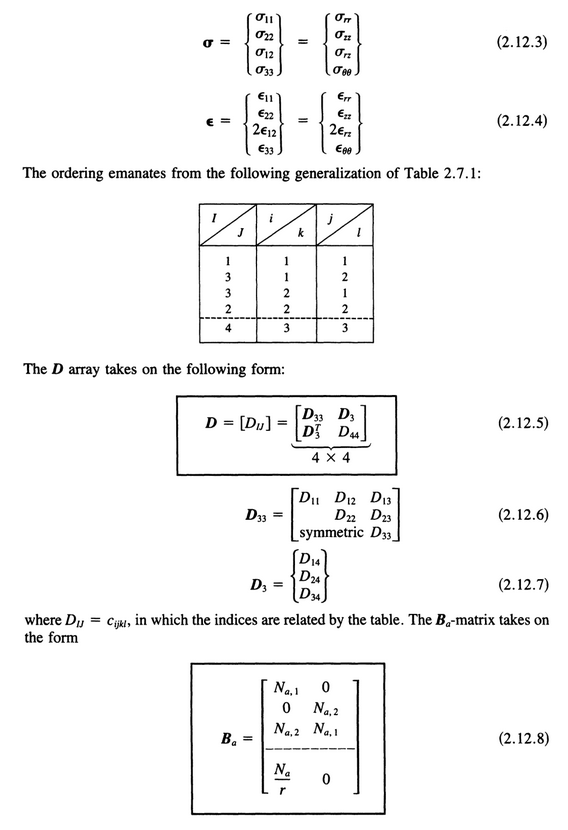
\includegraphics[width=10cm]{images/axisymmetry/hughes1}
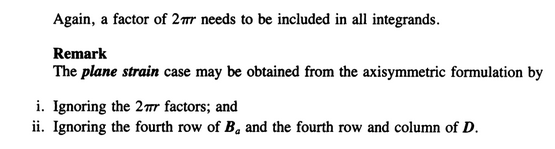
\includegraphics[width=10cm]{images/axisymmetry/hughes2}\\
{\captionfont Taken from pages 101 of \fullcite{hugh}.}
\end{center}


Also check page 469 of Gresho \& Sani's book, and 
see their remark on axisymmetric case for the N-S equations on page 545.

\Literature:
\begin{itemize}
\item \fullcite{ruas03}
\item \fullcite{leli12} 
\end{itemize}






